\section{Clasificación de equipos}

Tras la fase de calibración y proyección, el siguiente paso del pipeline consiste en identificar a qué equipo pertenece cada detección. El detector inicial permite diferenciar clases como jugador, portero, árbitro o balón, pero no proporciona directamente la pertenencia de equipo de cada futbolista. Para resolver esta limitación se implementa una fase específica de asignación basada en el color de la camiseta.

El planteamiento parte de una hipótesis sencilla: en un partido de fútbol, el rasgo visual más estable para distinguir a los jugadores de un equipo frente a los del rival es el color de la equipación. A partir de esta idea, la clasificación se divide en dos procesos: primero, la extracción del color representativo de la camiseta para cada detección candidata y después la asociación de ese color a uno de los dos equipos de campo presentes en el partido.

Todo este proceso se realiza en el espacio de color LAB. En este espacio, el canal $L$ representa la luminosidad, el canal $A$ codifica la oposición entre verde y rojo, y el canal $B$ codifica la oposición entre azul y amarillo. En la implementación de OpenCV estos valores se almacenan escalados en el rango $[0,255]$, con los canales $A$ y $B$ centrados aproximadamente en 128 para representar valores neutros. Se ha escogido LAB porque la distancia euclídea entre dos colores en este espacio se aproxima mejor a la diferencia perceptual que en RGB, lo que resulta útil para comparar colores de camisetas bajo distintas condiciones de iluminación. Aun así, este espacio no elimina por completo el efecto de sombras, reflejos o cambios de luz, especialmente porque el canal $L$ sigue dependiendo de la luminosidad de la imagen.

\subsection{Identificación del color de la camiseta}

La identificación del color de la camiseta parte de las cajas delimitadoras generadas por el detector. En la implementación se utilizan las coordenadas de la caja en formato $(x_1, y_1, x_2, y_2)$, que delimitan la región de la imagen donde se encuentra cada detección (jugador, portero o árbitro). Como la camiseta se encuentra normalmente en la parte superior del cuerpo, se recorta únicamente el 50\% superior del \textit{bounding box}. De esta forma se reduce la influencia del pantalón, las botas y parte del césped.

Esta aproximación no cubre todos los casos posibles. Por ejemplo, un jugador puede aparecer en el suelo, girado o parcialmente ocluido, pero estos casos son menos frecuentes y se asumen como excepciones dentro de un sistema que debe funcionar de forma robusta en la mayoría de frames.

Una vez extraída la región superior de la caja, todavía aparece un problema importante: el \textit{bounding box} es rectangular, mientras que el cuerpo del jugador no lo es. Por tanto, dentro del recorte no solo aparece la camiseta, sino también césped, cabeza, brazos u otros elementos de fondo. Para separar la camiseta del resto de píxeles se aplica KMeans con $k=2$ sobre los píxeles del recorte en espacio LAB. La idea es dividir los colores del recorte en dos grupos principales: uno correspondiente a la camiseta y otro correspondiente al fondo.

Aunque podrían plantearse más clusters, por ejemplo para separar cabeza, camiseta y césped, en la práctica $k=2$ ofrece un compromiso adecuado entre simplicidad, estabilidad y coste computacional. La cabeza o pequeñas regiones secundarias suelen quedar absorbidas por uno de los dos clusters, y su influencia sobre el centroide final es limitada si ocupan pocos píxeles frente a la camiseta o el fondo.

Para decidir qué cluster corresponde a la camiseta no se toma simplemente el cluster mayoritario, ya que en algunos recortes el fondo puede ocupar más superficie que el propio jugador. En su lugar, se selecciona un conjunto fijo de puntos de referencia del recorte (esquinas y bordes: superior-izquierda, superior-derecha, inferior-izquierda, inferior-derecha, centro superior, centro lateral izquierdo y centro lateral derecho). Estos puntos suelen pertenecer al fondo, por lo que el cluster más frecuente entre ellos se interpreta como fondo. El otro cluster se considera el de la camiseta, y su centroide LAB se guarda como color representativo de la detección.

\begin{equation}
\mathbf{c}_{\text{camiseta}} = [L, A, B]
\label{eq:color-camiseta-lab}
\end{equation}

Este proceso se aplica a cada detección (jugadores, árbitros y porteros). La decisión final de equipo y posibles reetiquetados de clase (por ejemplo, entre jugador, portero y árbitro) se realiza en la etapa de asociación descrita en el siguiente \hyperref[subsec:asociacionEquipo]{Apartado~\ref*{subsec:asociacionEquipo}}. En la \hyperref[fig:shirt-crop-kmeans]{Figura~\ref*{fig:shirt-crop-kmeans}} se muestra un ejemplo del recorte superior y la segmentación de color utilizada para estimar \(c_{camiseta}\).
\begin{figure}[H]
    \centering
    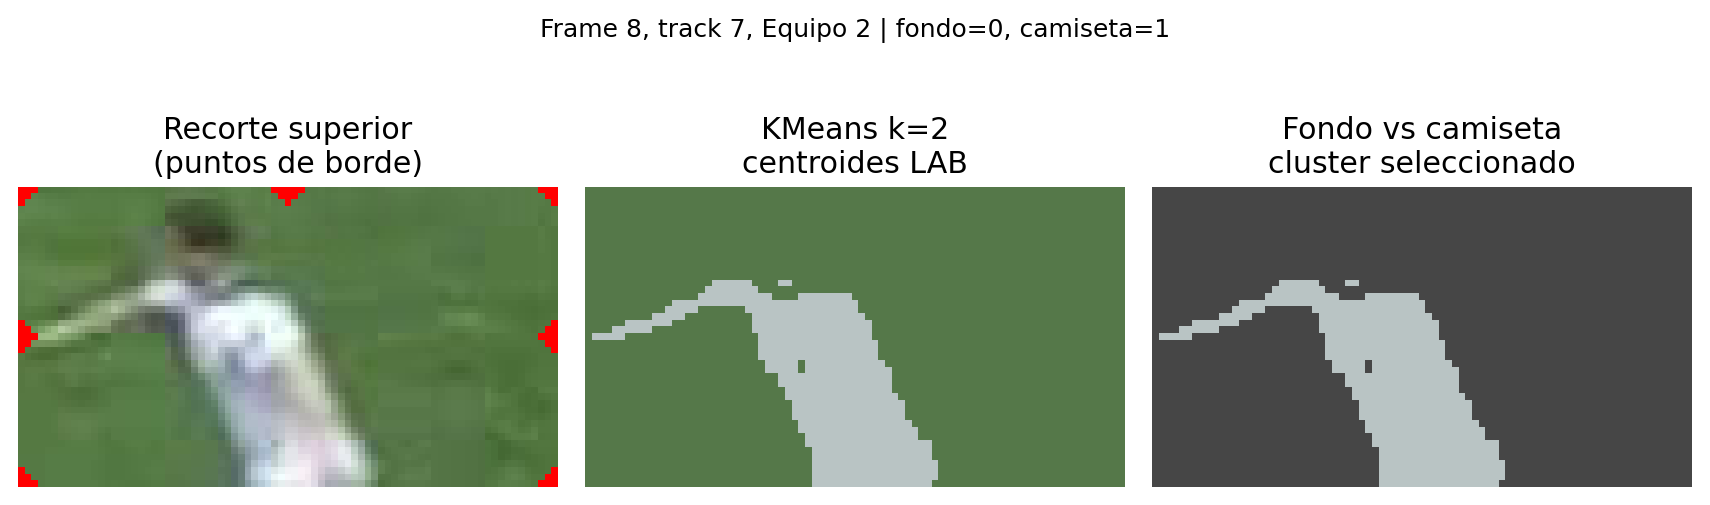
\includegraphics[width=0.9\textwidth]{Imagenes/Propias/shirt_crop_kmeans_example.png}
    \caption[Recorte de crop de jugador y KMeans]{Ejemplo de recorte superior de jugador y segmentación mediante KMeans con $k=2$.}
    \label{fig:shirt-crop-kmeans}
\end{figure}

\subsection{Asociación del equipo}
\label{subsec:asociacionEquipo}

En esta sección se describe la lógica para asociar cada track detectado a uno de los dos equipos.

\subsubsection{Asignación por color y centro del equipo}

Una vez obtenido el color de camiseta de cada detección candidata, representado por el vector $\mathbf{c}_{\text{camiseta}}$ definido en la Ecuación~\eqref{eq:color-camiseta-lab}, el objetivo es asociarlo a uno de los dos equipos de campo del partido. Para ello se acumulan muestras de colores LAB de las camistas de los jugadores y se aplica KMeans con $k=2$, esta vez no sobre píxeles individuales, sino sobre los colores de las camisetas ya extraídos. Cada cluster representa uno de los dos equipos de campo.

El centro de cada equipo se calcula mediante la mediana de las muestras LAB del cluster, en lugar de usar directamente la media. Esta decisión hace que la referencia de color sea más robusta frente a detecciones erróneas, sombras, reflejos o recortes en los que la camiseta no se haya aislado correctamente.

La asignación de una nueva detección se realiza calculando la distancia euclídea entre el color de su camiseta y el color de referencia de cada equipo:

\[
d(c, \mu_t) = \|c - \mu_t\|_2
\]

donde $c$ es el color LAB de la camiseta detectada y $\mu_t$ es el color representativo del equipo $t$. La detección se asigna al equipo cuya referencia esté más cerca:

\[
equipo(c) = \arg\min_t d(c, \mu_t)
\]


\subsubsection{Actualización online, \textit{bootstrap} y \textit{buckets} de muestras}

La construcción de clusters de color se realiza en modo online mediante un esquema de \textit{buckets} por clase, con dos contenedores principales: muestras de campo (\texttt{player}) y muestras de árbitro (\texttt{referee}). Cada nueva detección con color estimado solo se incorpora si supera una confianza mínima configurable.

Durante las primeras fases del vídeo, cuando los clusters de equipos todavía no están estabilizados, el sistema acumula muestras progresivamente y retrasa la actualización hasta disponer de soporte suficiente. Para el \textit{bucket} de jugadores, la actualización de centros no se lanza en cada frame, sino de forma periódica (cada 5 frames) y únicamente cuando se alcanza un mínimo de muestras acumuladas (en nuestra configuración, 60).

Cuando se ejecuta la actualización, se aplica KMeans con $k=2$ sobre las muestras LAB de jugadores. Después se valida el tamaño de los clusters obtenidos: si alguno resulta demasiado pequeño (por debajo de un mínimo configurable), se considera un cluster inválido, se descarta y se repite el ajuste sobre el cluster mayor. Si tras varias iteraciones no se obtiene una partición estable, la actualización se rechaza y se espera a nuevas muestras.

Además, para cada equipo se calculan estadísticas robustas de distancia intra-cluster (cuartiles e IQR), a partir de las cuales se define un umbral superior de pertenencia. Estas cotas se usan para detectar colores alejados del patrón esperado y limitar el impacto de \textit{outliers}.

En el caso del árbitro, el color de referencia no se estima con KMeans, sino mediante media recortada (\textit{trimmed mean}) sobre las muestras LAB acumuladas (recorte del 15\% por canal), lo que reduce la influencia de valores extremos y mejora la robustez del modelo.

En la \hyperref[fig:team-color-clusters-lab]{Figura~\ref*{fig:team-color-clusters-lab}} se puede ver como queda el estado de color de un partido después una ejecución. Se puede ver como el sistema es capaz de definir clusters bastante acertados sobre los colores de cada grupo de detecciones. Concretamente se puede ver el cluster del Equipo 1, de color verde, el cluster del Equipo 2, de color blanco, y el cluster de árbitros, de color negro. 

\begin{figure}[H]
    \centering
    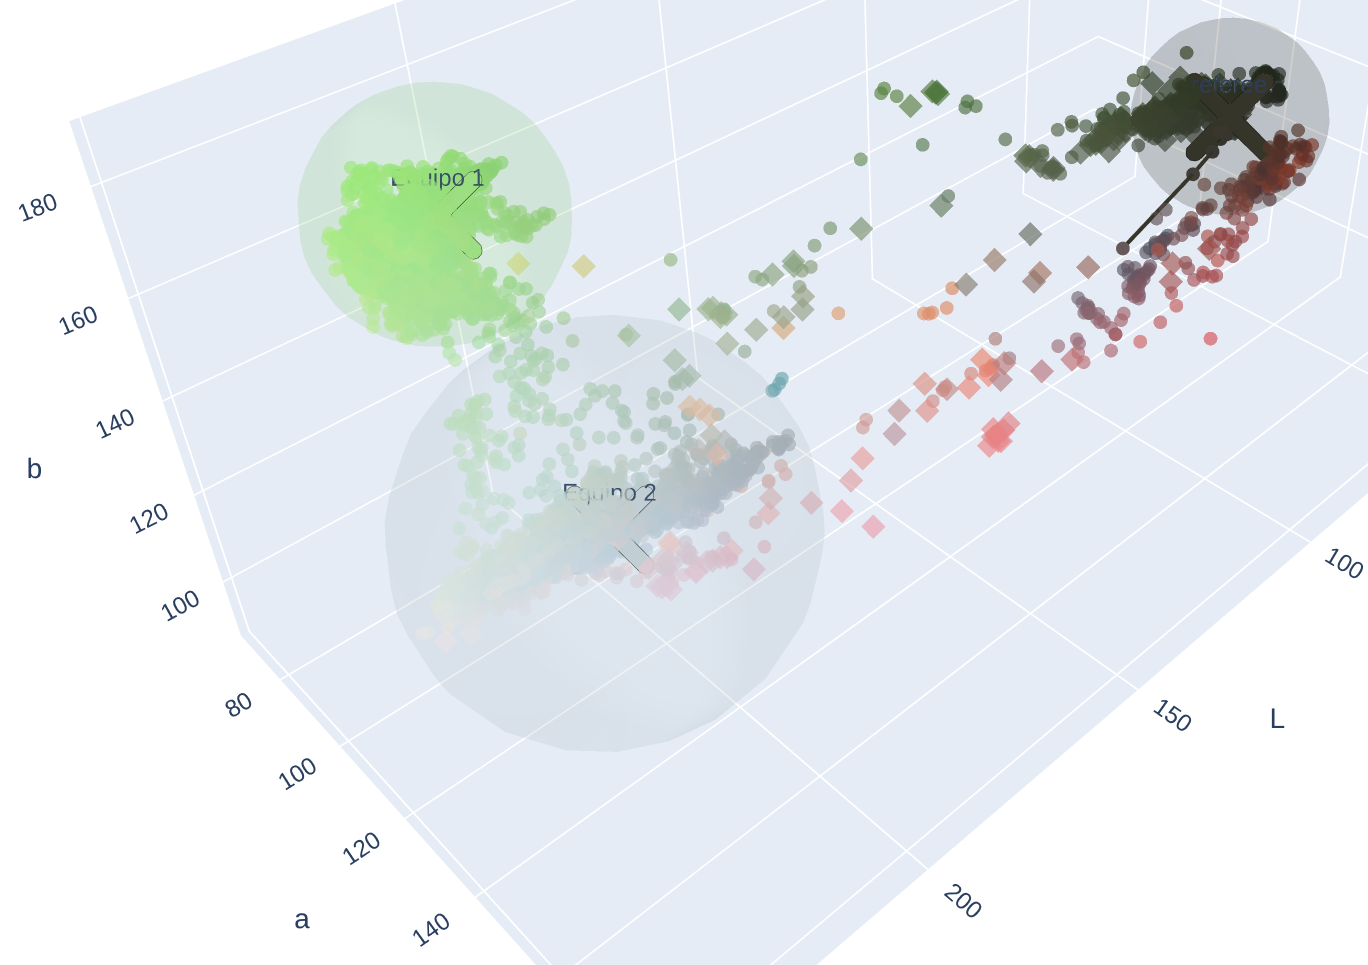
\includegraphics[width=0.7\textwidth]{Imagenes/Propias//lab_scatter_3d.png}
    \caption[Distribución de detecciones en el espacio LAB]{Distribución de detecciones en el espacio LAB, referencias de color y fronteras de pertenencia por equipo.}
    \label{fig:team-color-clusters-lab}
\end{figure}

\subsubsection{Reetiquetado de clase}

Una vez disponible el estado de color (centros de equipo, referencia de árbitro y umbrales de pertenencia), la inferencia por detección no se limita a asignar equipo: también puede reajustar la clase semántica final de la detección. En concreto, para cada candidato con color de camiseta estimado se calcula su distancia a los centros disponibles y, junto con restricciones posicionales en coordenadas de campo, se decide la etiqueta final entre \texttt{player}, \texttt{referee} y \texttt{goalkeeper}.

Si el color se asocia al patrón de árbitro, la detección solo se confirma como \texttt{referee} cuando también supera las compuertas posicionales definidas para ese rol (estar pegado a las líneas de banda o en una posición central del campo).

Cuando una detección queda fuera del patrón de equipos de campo pero su posición es compatible con portero, puede reetiquetarse como \texttt{goalkeeper}.

Para jugadores de campo, la pertenencia a equipo se valida además con umbrales robustos intra-cluster (derivados de cuartiles e IQR). Así, una detección no se acepta únicamente por vecino más cercano, sino también por consistencia estadística con el cluster de destino. 

En resumen, la salida de esta fase no es solo un color asignado a un equipo, sino una decisión conjunta \textit{clase + equipo} condicionada por evidencia cromática y geométrica, lo que mejora la robustez frente a confusiones entre jugador, árbitro y portero.

La \hyperref[fig:field-relabel-map]{Figura~\ref*{fig:field-relabel-map}} muestra el funcionamiento del re-etiquetado sobre coordenadas de campo. En naranja se representan los casos en los que una detección inicial de \texttt{player} se reclasifica como \texttt{referee}, y en azul los casos \texttt{player}$\rightarrow$\texttt{goalkeeper}. La distribución espacial de estos puntos coincide con lo que se observa en el vídeo de referencia: los re-etiquetados naranjas se concentran en la zona central, consistente con la trayectoria del árbitro principal, mientras que los re-etiquetados azules aparecen en el entorno del área izquierda, compatible con la posición típica de un portero. Además, los cambios se producen únicamente dentro de las regiones de validez definidas por las compuertas posicionales de cada clase.


\begin{figure}[H]
    \centering
    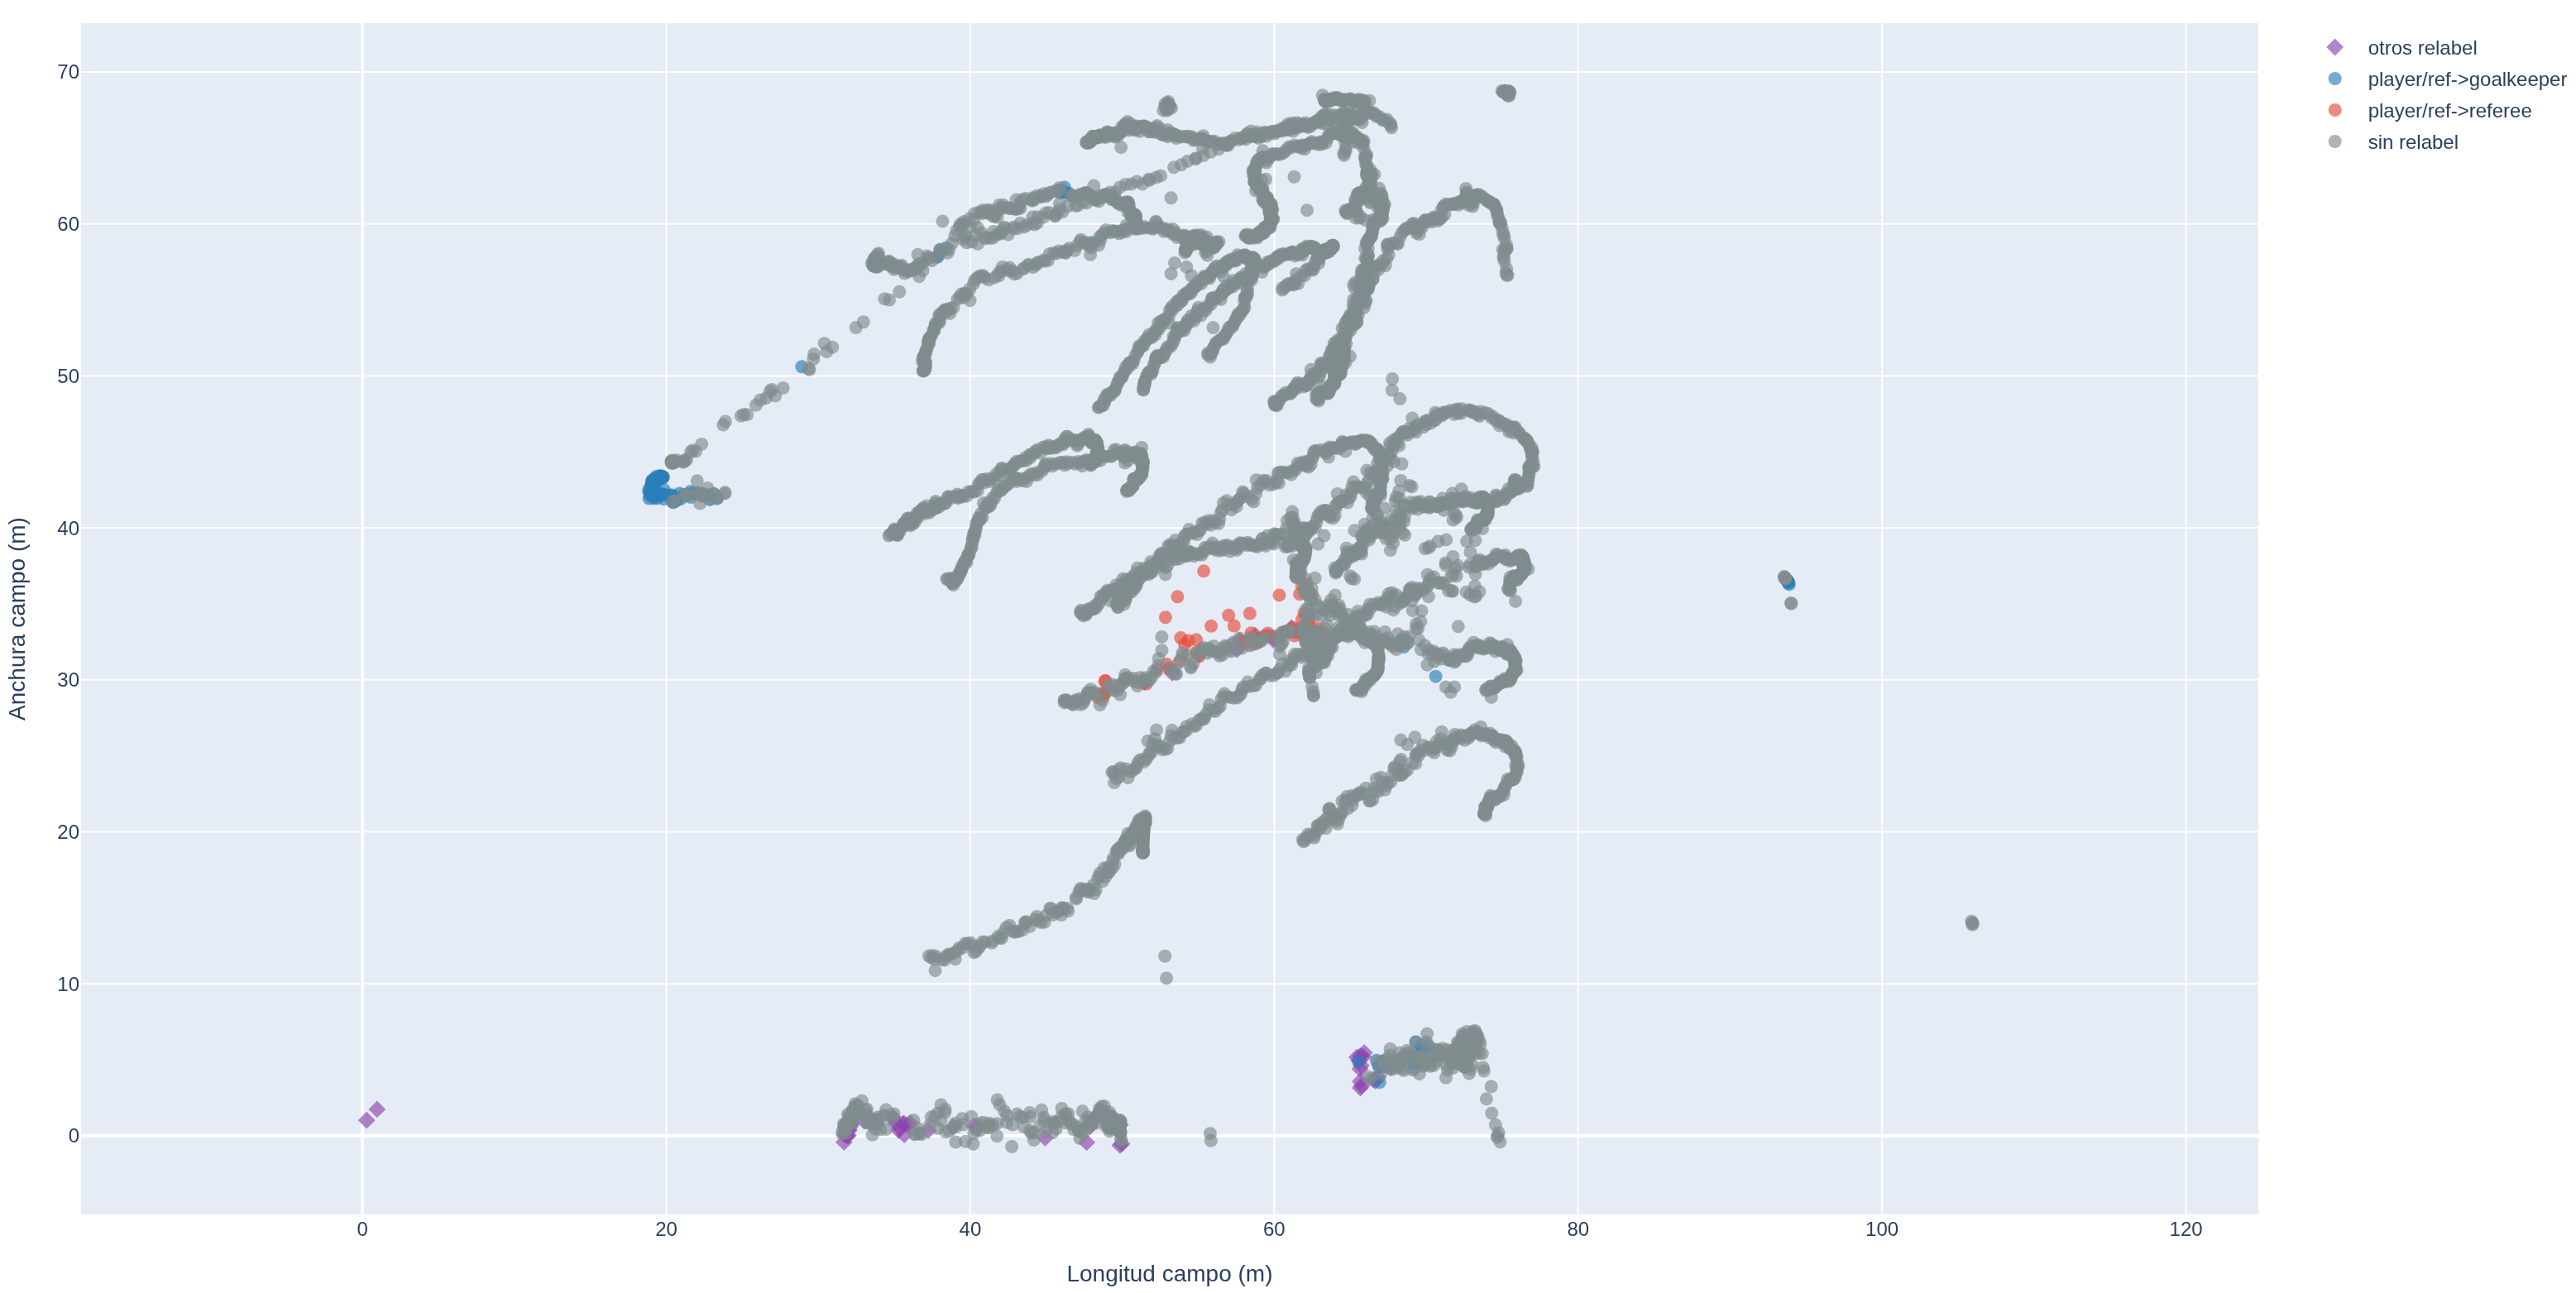
\includegraphics[width=0.95\textwidth]{Imagenes/Propias/field_relabel_map.png}
    \caption[Mapa de relabels en el campo]{Mapa de posiciones en campo con casos de relabel por categoría.}
    \label{fig:field-relabel-map}
\end{figure}


La configuración operativa del módulo se resume en la Tabla~\ref{tab:clasificacion_equipos}. 
\begin{table}[htbp]
    \centering
    \begin{tabular}{c|c}
        \textbf{Parámetro} & \textbf{Valor utilizado} \\
        \hline\hline
        Espacio de color & LAB \\
        Región analizada & 50\% superior del bounding box \\
        Clusters para camiseta & 2 \\
        Clusters para equipos de campo & 2 \\
        Muestras mínimas (\texttt{player}) & 60 acumuladas \\
        Muestras mínimas (\texttt{referee}) & 15 acumuladas \\
        Frecuencia de actualización de clusters & cada 5 frames \\
        Tamaño mínimo de cluster (\texttt{min\_size\_cluster}) & 15 \\
        Centro de equipo & mediana LAB del cluster \\
        Referencia de árbitro & \textit{trimmed mean} LAB (15\%) \\
        Distancia de asignación & euclídea en LAB \\
        \hline
    \end{tabular}
    \caption{Configuración principal del módulo de clasificación de equipos.}
    \label{tab:clasificacion_equipos}
\end{table}

Finalmente, cabe destacar que esta fase fue uno de los cuellos de botella iniciales del pipeline. En una primera versión, el clustering de cada camiseta se realizaba en CPU con \texttt{scikit-learn}, lo que incrementaba el tiempo de procesamiento por frame. Para reducir esta latencia se implementó una versión batched del KMeans con aceleración en GPU cuando está disponible (basada en \texttt{CuPy}), manteniendo \texttt{scikit-learn} como alternativa en CPU. En nuestras pruebas, esta optimización redujo el tiempo aproximado de identificación de camisetas y asignación de equipo de 1.5 s/frame a 0.05 s/frame, lo que supone una aceleración de aproximadamente $30\times$.

